\documentclass[11pt, oneside]{article}   	% use "amsart" instead of "article" for AMSLaTeX format
\usepackage{geometry}                		% See geometry.pdf to learn the layout options. There are lots.
\geometry{letterpaper}                   		% ... or a4paper or a5paper or ... 
%\geometry{landscape}                		% Activate for for rotated page geometry
%\usepackage[parfill]{parskip}    		% Activate to begin paragraphs with an empty line rather than an indent
\usepackage{graphicx}				% Use pdf, png, jpg, or eps§ with pdflatex; use eps in DVI mode
								% TeX will automatically convert eps --> pdf in pdflatex		
\usepackage{amssymb}
\usepackage{amsmath}
\usepackage{parskip}
\usepackage{color}
\usepackage{hyperref}

\title{Gaussian integral}
%\author{The Author}
%\section{}
%\subsection*{}
\date{}							% Activate to display a given date or no date

\graphicspath{{/Users/telliott_admin/Dropbox/Tex/png/}}
% \begin{center} 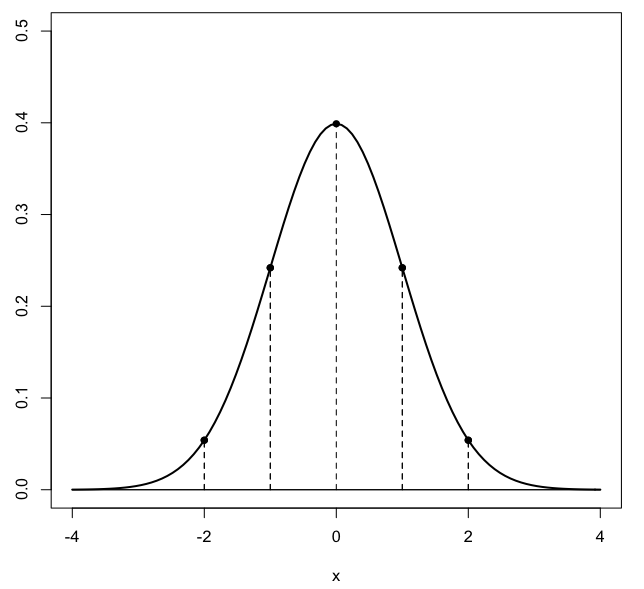
\includegraphics [scale=0.4] {gauss3.png} \end{center}
\begin{document}
\maketitle
\Large
The Gaussian or normal distribution is a central tool in probability and statistics.  The distribution has the form:
\[ p(x) = \int e^{-(x-\mu)^2/2 \sigma^2} \ dx \]
where $\mu$ is the mean and $\sigma^2$ the variance, which determine the placement and shape of the bell. The square root of the variance is $\sigma$, the standard deviation.  We will assume for what follows that $x$ has been centered so that the mean is equal to zero.

An important result is that there is no way to solve this integral in the usual sense, that is, no "closed form" exists.  One simply integrates numerically over an interval $[a,b]$ to obtain the probability that the random variable $x$ lies in the interval ($a \le x \le b$).

Remarkably it \emph{is} possible to derive a value for the integral when the interval is $[-\infty,\infty]$, and even more remarkably, the value is $\sqrt{2 \pi} \cdot \sigma$.  This leads to writing the "normalized" distribution so that the probability sums to $1$ as
\[ \frac{1}{\sqrt{2 \pi} \cdot \sigma}  \int e^{-(x-\mu)^2/2 \sigma^2} \ dx \]
(alternatively, put $\sigma^2$ under the square root).

Here is a neat and fairly simple proof that the value of the integral given above is correct.  It is based on integrating a volume.  

We will show that
\[ \int_{-\infty}^{\infty} e^{-kx^2} \ dx = \sqrt{\frac{\pi}{k}} \]

The trick is to imagine the surface that is formed by rotating this function around the $z$ axis in three-dimensions.  It looks like this:

\begin{center} 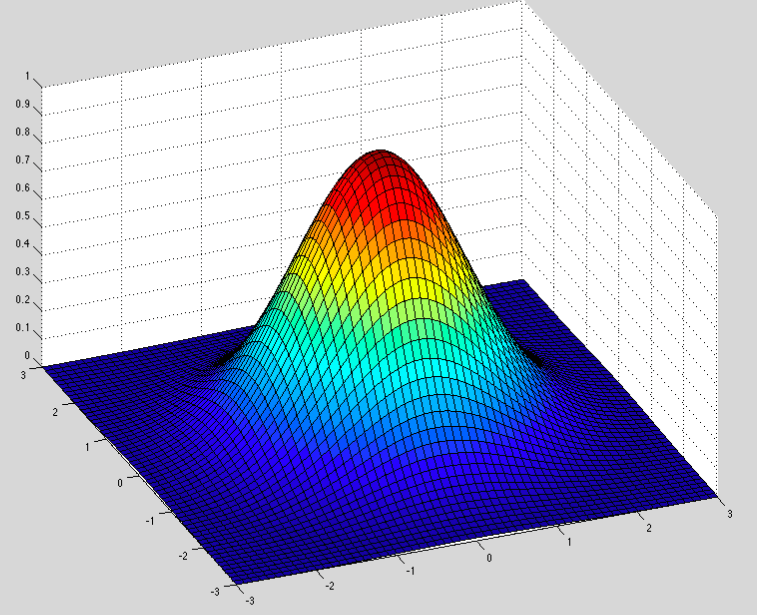
\includegraphics [scale=0.35] {gaussian-surface.png} \end{center}
The volume is contained under the surface and above the $xy$-plane.  It's a real bell!

The equation of this surface is like two perpendicular copies of the gaussian:
\[ z = e^{-(x^2 + y^2)/2} \]
For any constant value of $y$ like $y=0$ we have the standard normal function for $x$ (with standard deviation equal to $1$), and vice-versa.  (In fact, any vertical slice that includes the origin is a standard normal).

We compute the volume under the surface in two ways.  The first way is by horizontal slices perpendicular to the $z$-axis.

\subsection*{Horizontal slices}
\[ \int_0^b A(z) \ dz \]

We need an expression for the area of horizontal slices as a function of the height $z$.  What we have now is the inverse function:
\[ z = e^{-k(x^2 + y^2)} \]
(I am using $k$ now rather than $1/2$ to make the result more general).

So let's invert it:
\[ x^2 + y^2 = -\frac{1}{k} \ \ln z \]
The horizontal cross-sections (at $z = c$, with $c$ a constant), are circles of radius $r$: where
\[ r^2 = x^2 + y^2 = -\frac{1}{k} \ \ln z \]
The area, $A = \pi r^2$:
\[ A(z) = \pi \ \frac{- \ln z}{k}  \]

We will fix the upper bound as follows:  the maximum value of $z$ occurs when $x=y=0$ so the exponential is equal to $1$, otherwise the value is less than $1$, so we have that 
\[  b = e^{-(x^2 + y^2)/2} = e^0 = 1 \]
This will be the upper bound on $z$ when we calculate the volume.
\[ V = -\frac{\pi}{k} \int_0^1 \ln z \ dz \]

Put the leading factor aside for now and consider
\[ \int \ln z \ dz = z \ln z - z \]
which is easily verified by differentiating.

We need to evaluate this expression between the bounds we set above ($z=0 \rightarrow 1$).  At the upper bound, the first term is zero and the second is equal to $-1$.

At the lower bound of $z=0$, clearly the second term is zero.
  
The problem is the first term, $z \ \ln z$.  To evaluate this, consider the limit
\[ \lim_{z \rightarrow 0+}  z \ \ln z  \]
 
\[ = \lim_{z \rightarrow 0+}   \frac{z}{1/\ln z} \]

As $z \rightarrow 0+$, the numerator is just zero and the denominator is :$1/-\infty = 0$.  We use L'Hopital's rule.  Compute the derivatives:
\[ \lim_{z \rightarrow 0+} \frac{1}{1/(1/z)} = \lim_{z \rightarrow 0+} z = 0 \]
As this limit is equal to zero we have just zero for the whole expression at the lower bound.

Remembering the extra factor, we have finally $(-\pi/k)(-1) = \pi/k$.  (The factor of $-1$ is there because we are subtracting the value at the lower bound).

\subsection*{Vertical}
The other way is vertical slices.  First, label the value of the integral, which we seek, as $I$:
\[ I = \int_{-\infty}^{\infty} e^{-kx^2} \ dx \]

Again, $I$ is what we're looking for.  It is \textbf{just a number}.  

Our function is
\[ z = e^{-k(x^2 + y^2)} \]
If we take slices perpendicular to the $x$-axis (with $x =$ constant for any particular slice), the area of each slice is
\[ A(y) = \int_{-\infty}^{\infty} e^{-k(x^2 + y^2)} \ dy \]
since  $x$ is a constant we have
\[ = e^{-kx^2} \ \int_{-\infty}^{\infty} e^{-ky^2} \ dy = e^{-kx^2} \ I \]

Now we add up all the little slices to find the volume, which is
\[  V =  \int_{-\infty}^{\infty} I e^{-x^2/2} \ dx \]
but $I$ is just a number, so
\[  =  I \int_{-\infty}^{\infty} e^{-x^2/2} \ dx \]
\[ = I^2 \]

Alternatively, just say that $x$ and $y$ are independent so that
\[ \iint e^{-kx^2} e^{-ky^2} \ dy \ dx \]
\[ = \int e^{-kx^2} \ dx \int e^{-ky^2} \ dy = I^2 \]

Now we have two different expressions for the same volume, which must then be equal to each other.  Thus:
\[ \frac{\pi}{k} = I^2 \]
\[ I = \sqrt{\frac{\pi}{k}} \]
Thinking about the formula that contains a $2$ and the variance $\sigma^2$ in the denominator of the exponential, $1/k = 2 \sigma^2$ so
\[ I = \sqrt{2 \pi \sigma^2 }   = \sqrt{2 \pi } \cdot \sigma \]
We \emph{divide} by this in order to normalize, to make the value of the whole integral be equal to $1$, as it must for a probability distribution.

\subsection*{Change of variables}
Taking another look at the bell, we see that we can change variables and do this even faster, not worrying about the horizontal slices.

$x^2 + y^2 = r^2$ so
\[ \int_{-\infty}^{\infty} \int_{-\infty}^{\infty} e^{-kx^2} e^{-ky^2} \ dy \ dx = \int_{\theta = 0}^{2 \pi} \int_{r=0}^{\infty} e^{-kr^2} r \ dr \ d \theta \]
The $r$ is there because of the switch to polar coordinates.  (Careful with the bounds on $r$!).  It makes the integral easy
\[  \int_{0}^{\infty} e^{-kr^2} r \ dr  = -\frac{1}{2k} e^{-kr^2} \ \bigg |_0^{\infty} \]
The negative exponential is zero at the upper bound and $1$ at the lower one.  We pick up a factor of $2 \pi$ from integrating with respect to $\theta$.  So finally we have just
\[ 2 \pi \cdot \frac{1}{2k} = \frac{\pi}{k} \]
which is equal to $I^2$ as we argued before.

\end{document}  